\section{Experimental Results in the 14T Magnetic Field}
\label{sec:bts:result14T}





%%%%%%%%%%%%%%%%%%%%%%%%%%%%%%%%%%%%%%%%
%%%%%%%%%%%%%%%%%%%%%%%%%%%%%%%%%%%%%%%%
%%%%%%%%%%%%%%%%%%%%%%%%%%%%%%%%%%%%%%%%
%%%%%%%%%%%%%%%%%%%%%%%%%%%%%%%%%%%%%%%% FIGURE 1

%The ARPES experiments by Hasan's group ~\cite{BTS_ARPES} have shown that Bi$_2$Te$_2$Se has a single Dirac cone on the surface. Since Bi$_2$Se$_3$ crystals are $n$-type due to the Se vacancies and Bi$_2$Te$_3$ is $p$-type due to the Bi-Te anti-site defects. We are motivated to grow crystals of Bi$_2$Te$_2$Se so that both dopants could be compensated by each other in order to reduce the total bulk carriers. More specifically, 

To find the composition for optimal compensation, we first grew a series of hybrid semiconductors Bi$_2$Te$_{2-x}$Se$_{1+x}$ and made some test measurements to find the composition that yields the lowest carrier density. The thermopower signal is a good sign for the carrier type, and Bi$_2$Se$_3$ has a negative thermopower and Bi$_2$Te$_3$ displays a positive thermopower. Therefore we also used the thermopower signal to search for the optimal composition. We found that the low-temperature thermopower varies systematically, reflecting changes in $E_F$. 

The first generation of Bi$_2$Te$_2$Se crystals in our experiments were grown by a modified Bridgeman method from high purity elemental starting materials. We heated a mixture of stoichiometric Bi, Te and Se elements for one day at 850 $^{\circ}$C in a clean evacuated quartz tube, the melt was cooled to 500 $^{\circ}$C in a temperature gradient and then it was left to anneal for 2 days before cooling rapidly to the room temperature. To mount the contacts, we carefully cleaved the crystals with a razor blade and got a thin piece with a shiny surface. Then we attached contacts using silver paint, and then loaded the sample into the cryostat. We tried to minimize the time of this process so that the fresh surface experiences minimum hazard from oxidization. For the sample reported here, the crystal thickness is $d$ = 110 $\mu$m, while the distance between voltage leads equals 0.5 mm.  Fig. \ref{figRvsT_lo}A shows the resistivity v.s. temperature profile measured at $B$ = 0. Above 60K, it has a steep increase as the temperature drops, indicating that $E_F$ is in the bulk band gap. Below 40 K, the value of $\rho$ starts to saturate and attains values in the range 5-6 $\Omega$cm, or $\sim$1000 times higher than in non-metallic Bi$_2$Te$_3$. Converted to an areal resistance $R_{\square}= \rho/d$, the low-$T$ resistance corresponds to $R_{\square}$ = 400 $\Omega$. The Hall coefficient $R_H$ below 10 K is negative and implies a very small $n$-type bulk carrier density $n_b\sim 2.6\times 10^{16}$ cm$^{-3}$. From the Hall density and the observed $\rho$ together, we obtain a low bulk mobility $\mu_b\sim$ 50 cm$^2$/Vs.

\begin{figure}[!htbp]
  \begin{center}            
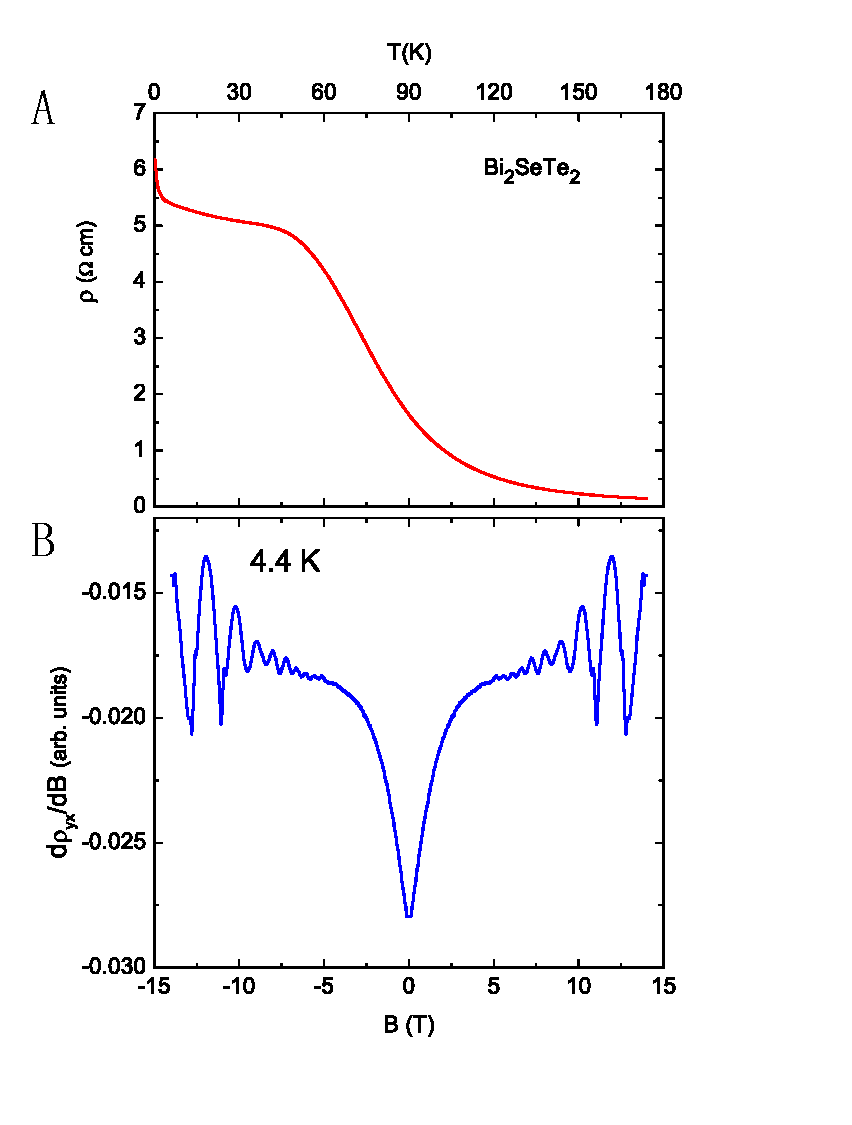
\includegraphics[width=0.9\linewidth]{ch-bts/figures/FigRvsT_lo.pdf} 
\caption{\label{figRvsT_lo}
The resistivity v.s. temperature curve and the derivative of the magnetoresistance curve of the bulk-insulating TI Bi$_2$Te$_2$Se.
Panel (A) shows $\rho$ vs. $T$ measured in $B$ = 0.  Below 10 K, $\rho$ 
reaches as high as 5.5 $\Omega$cm, or an areal
resistance $R_{\square}$ = 400 $\Omega$.  It was one of the most insulating TI crystals. The large resistivity indicates a very low bulk carrier density. Despite the non-metallic
value of $R_{\square}$, sizeable quantum oscillations are observed below 38 K.
Panel (B) displays the prominent SdH oscillations observed 
in the derivative $d\rho_{xy}/dB$ vs. $B$ at 4.4 K. Compared to Bi$_2$Te$_3$, the much larger SdH oscillations in Bi$_2$Te$_2$Se indicate a larger surface proportion of the current in the sample.
} 
  \end{center}
\end{figure}

A powerful way to study the properties of the energy band in a crystal is through the Shubnikovde Haas (SdH) oscillations in the magnetoresistance. High-quality SdH oscillations can uncover a lot of important information, such as the Fermi surface and the mobility of the bands. However, the sample needs to have a high mobility to generate SdH oscillations. In general, a sample with $\mu_b$ as low as 50 cm$^2$/Vs should not display Shubnikovde Haas oscillations in a magnetic field less than 14T. Surprisingly, however, the Hall resistivity $\rho_{yx}$ of our Bi$_2$Te$_2$Se sample displays prominent SdH oscillations that is resolved up to 38 K and down to 5 T. We have detected SdH oscillations in several crystals of Bi$_2$Te$_2$Se with $\rho$-$T$ profiles similar to that in Fig. \ref{figRvsT_lo}A. To emphasize the SdH oscillations, we display the the derivative $d\rho_{yx}/dT$ vs. $B$ at $T$ = 4.4 K in Fig. \ref{figRvsT_lo}B. It clear shows the high quality of the SdH oscillations. Independently, SdH oscillations were also observed in Bi$_2$Te$_2$Se by Y. Ando group~\cite{Ando10}. Since the bulk has a low mobility that could not generate SdH oscillations, we believe that the SdH oscillations originate from the surface states. We will discuss the analysis and reasons below. The work by Ren \etal~\cite{Ando10} also provides solid evidence the surface nature of the SdH oscillations by tracing the Fermi surface area in a tilted magnetic field.

Since the bulk still has a large carrier density, we believe that comparable surface conductance and bulk conductance coexist as parallel charge transport channels in Bi$_2$Te$_2$Se. To separate the bulk and surface contribution in the resistance measurement, it is convenient to convert resistance to conductance for the analysis. Since the total conductance $G$ is additive for parallel channels, the observed conductivity $\sigma_{ij}$ is
then the sum
\be
\sigma_{ij} = \sigma^b_{ij} + G^s_{ij}/d,
\label{eq:sigma}
\ee
where $\sigma^b_{ij}$ is the bulk conductivity and $G^s_{ij}$ is the conductance matrix of the surface states. The conductivity matrix $\sigma_{ij}$ is obtained by inverting the resistivity matrix $\rho_{ij}$. To isolate the SdH oscillations from the surface contribution in $\sigma_{xy}$, we define 
$\Delta\sigma_{xy} = \sigma_{xy} - \langle\sigma_{xy}\rangle$, where $\langle\sigma_{xy}\rangle$ is a smooth background. Here we use a low-power polynomial function to simulate and fit the background curve.


%%%%%%%%%%%%%%%%%%%%%%%%%%%%%%%%%%%%%%%%
%%%%%%%%%%%%%%%%%%%%%%%%%%%%%%%%%%%%%%%%
%%%%%%%%%%%%%%%%%%%%%%%%%%%%%%%%%%%%%%%%
%%%%%%%%%%%%%%%%%%%%%%%%%%%%%%%%%%%%%%%% FIGURE 

\begin{figure}[!htbp]
  \begin{center}            
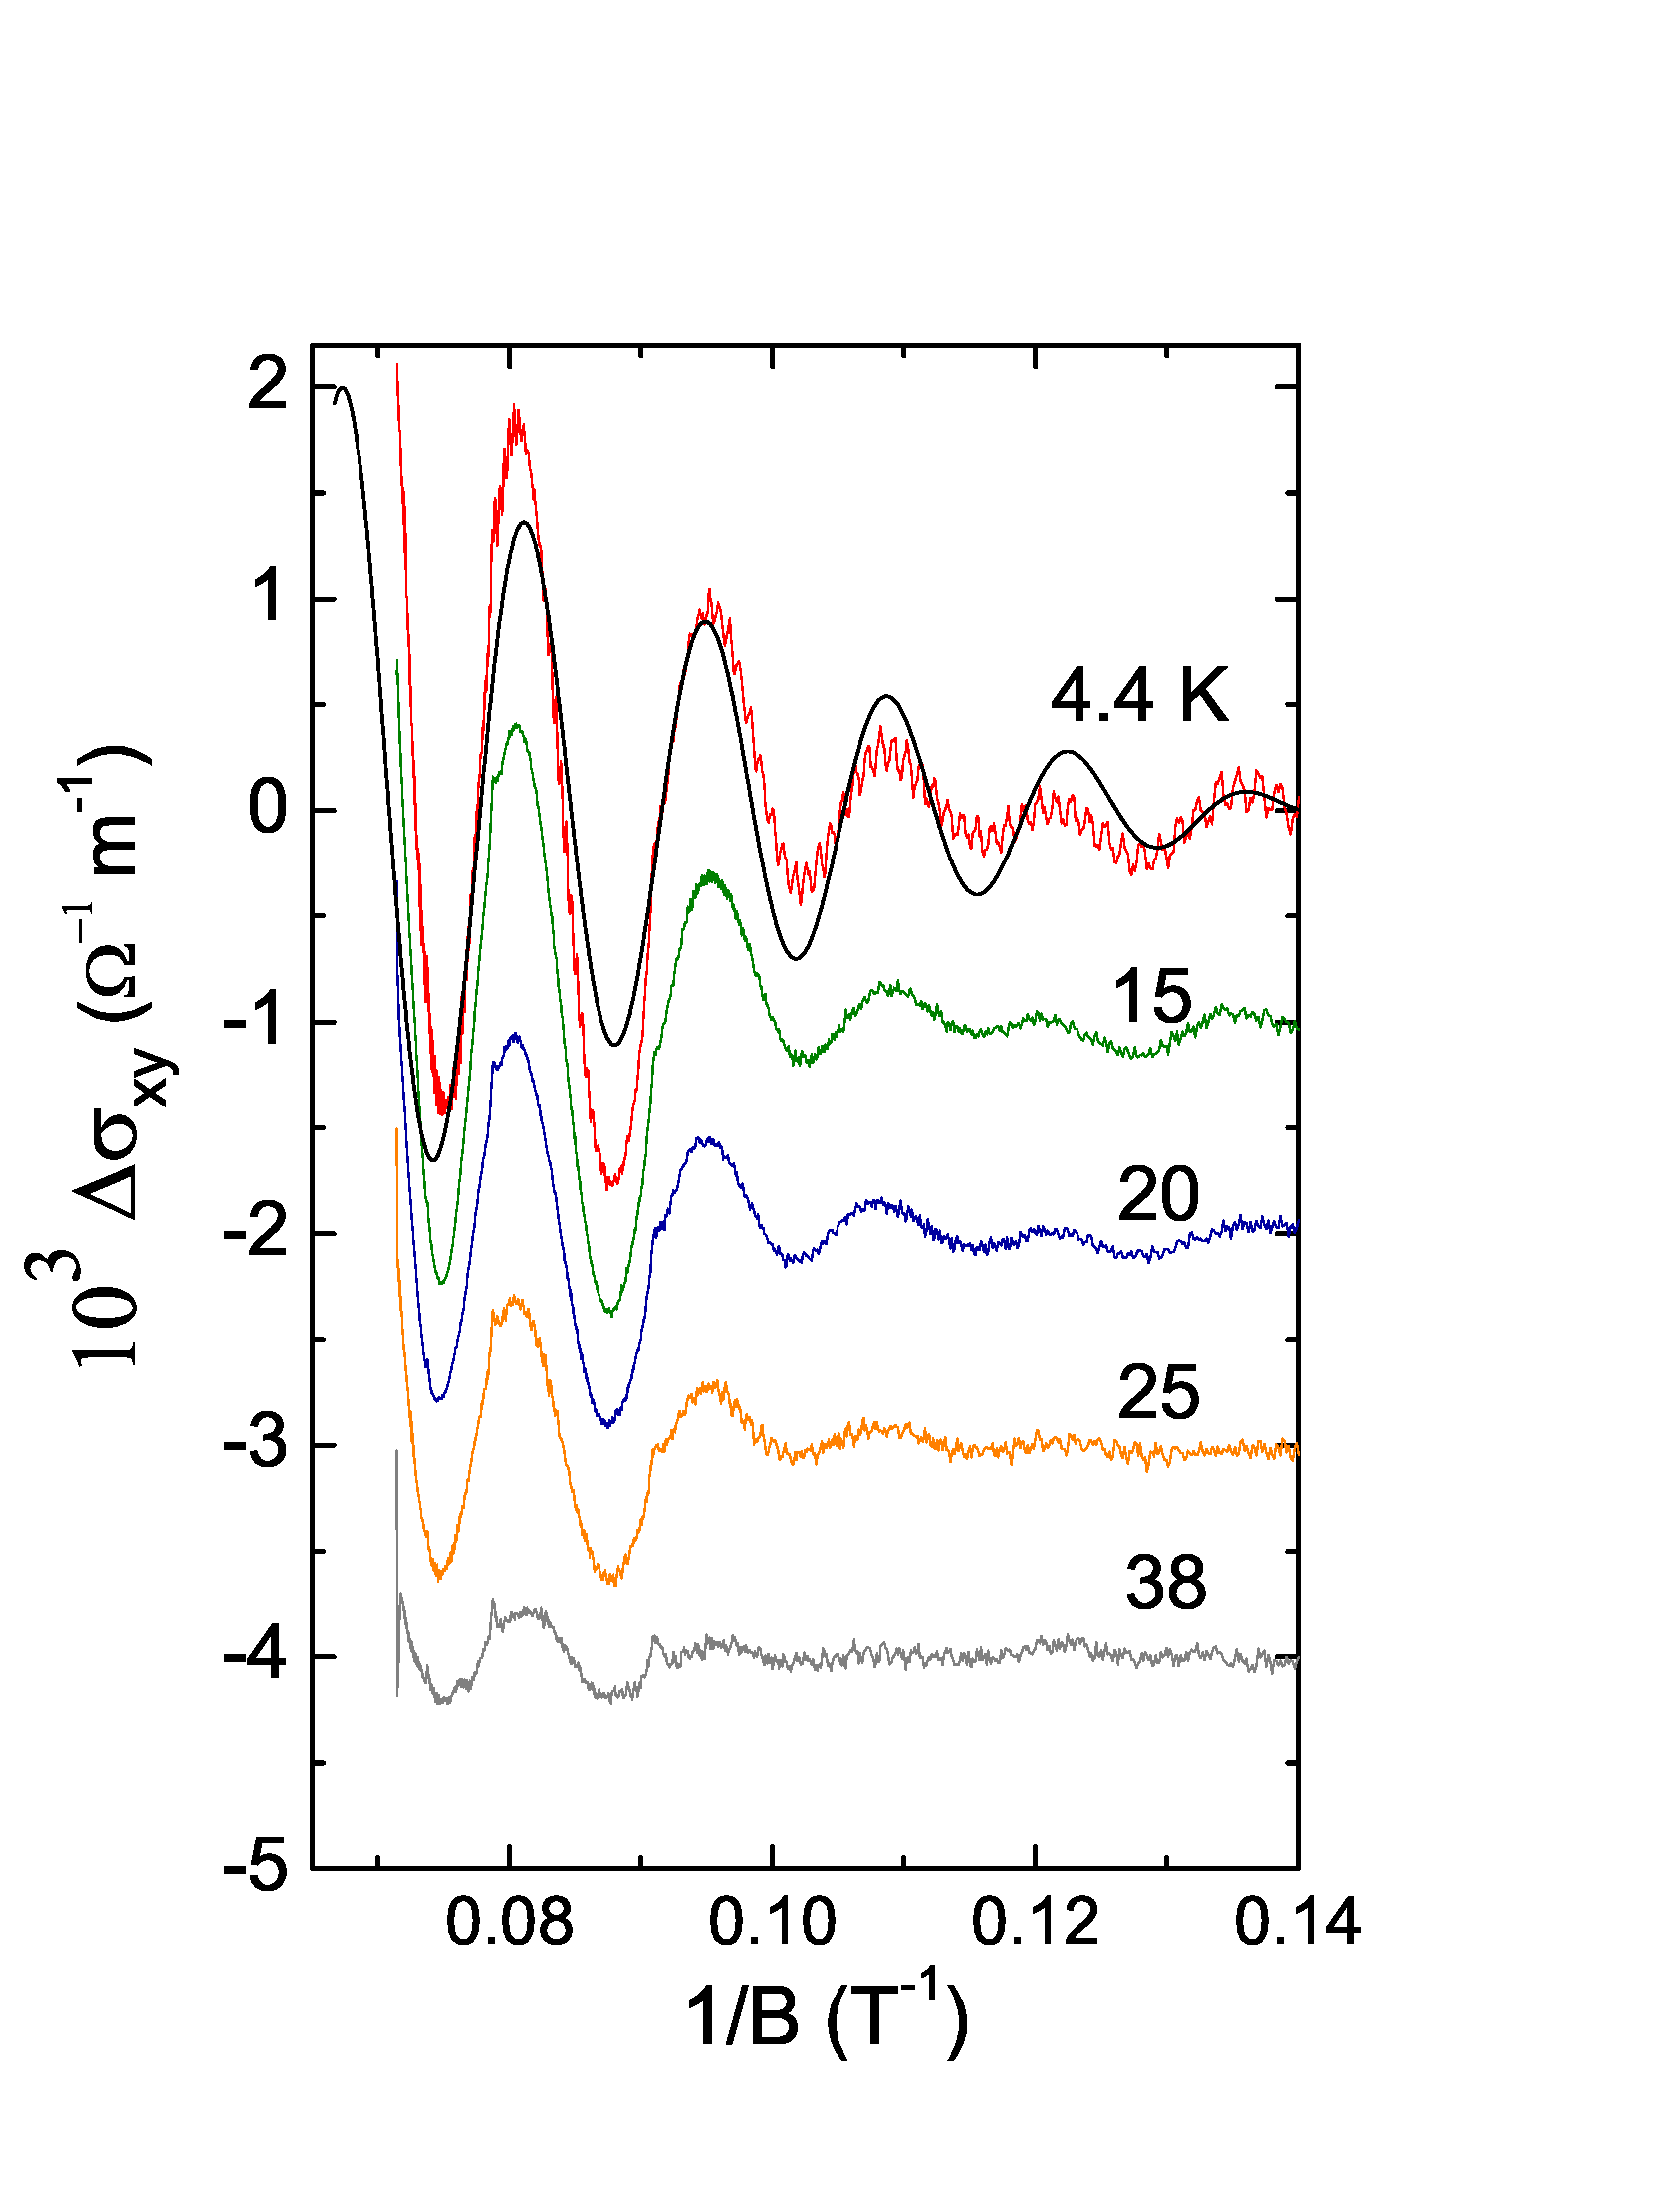
\includegraphics[width=0.9\linewidth]{ch-bts/figures/FigsxyT.eps}
\caption{\label{figsxy} 
Traces of the Hall conductivity $\Delta\sigma_{xy}$ 
(background subtracted) versus $1/B$ at selected $T$ for Bi$_2$Te$_2$Se.
The amplitudes of the oscillations decrease with an increasing $T$ but are still resolvable to 38 K.  
The smooth curve in the uppermost trace is a fit to $\Delta\sigma_{xy}$ by at 4.4 K 
using Eq. \ref{eq:sdh_hall}. The rapid decrease of the oscillation amplitudes for $1/B>$ 0.09 T$^{-1}$
reflects possible interference between 2 terms of similar amplitudes but slightly different
densities ($n_{s1},\;n_{s2}$) = (1.8, 1.7)$\times 10^{12}$ cm$^{-2}$.  
The fit yields the mobility $\mu$ = 2,800 cm$^2$/Vs and $k_F\ell$ = 41.This mobility is much higher than the one we obtained from the $\rho$ and the Hall density. Thus it indicates a different origin from the bulk states.
}
  \end{center}
\end{figure}


%%%%%%%%%%%%%%%%%%%%%%%%%%%%%%%%%%%%%%%%
%%%%%%%%%%%%%%%%%%%%%%%%%%%%%%%%%%%%%%%%
%%%%%%%%%%%%%%%%%%%%%%%%%%%%%%%%%%%%%%%%
%%%%%%%%%%%%%%%%%%%%%%%%%%%%%%%%%%%%%%%% FIGURE

\begin{figure}[!htbp]
  \begin{center}            
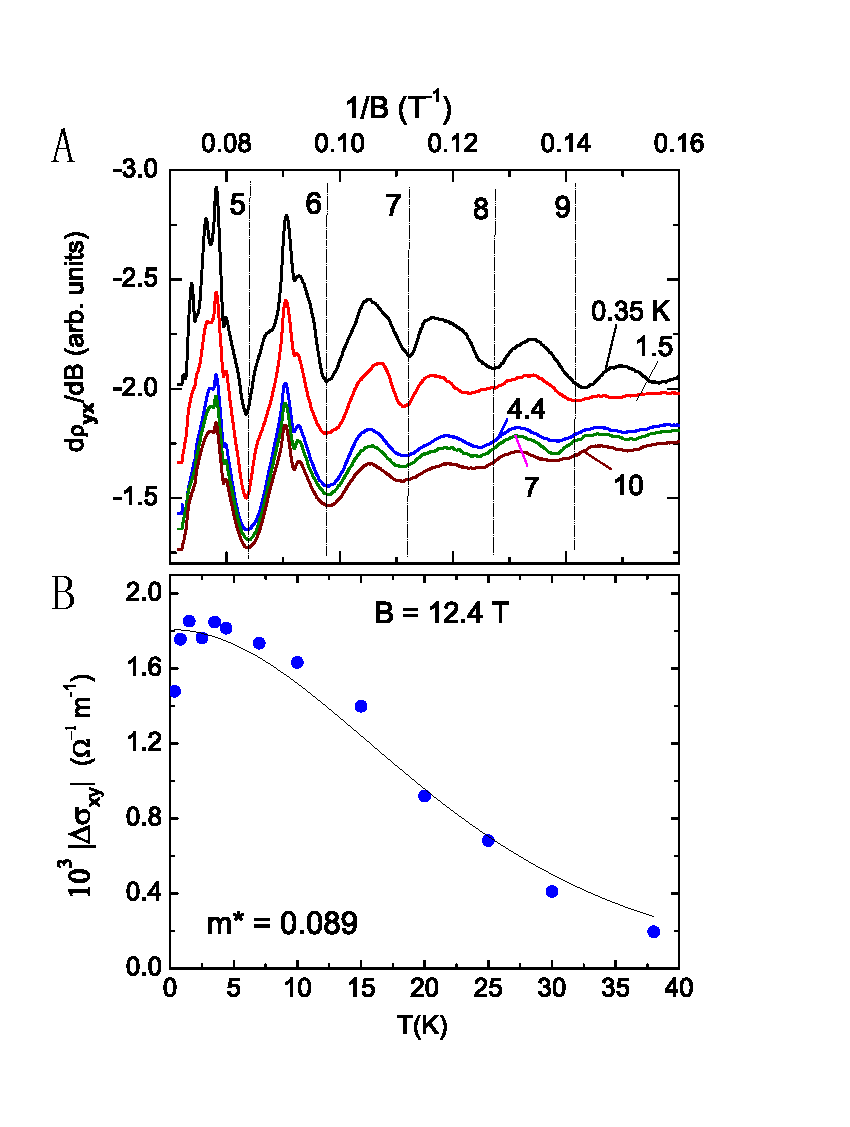
\includegraphics[width=0.9\linewidth]{ch-bts/figures/FigFitvsTemp.pdf} 
\caption{\label{figfit} (Color online) 
Panel (A) displays traces of the Hall resistivity 
$d\rho_{yx}/dB$ in Bi$_2$Te$_2$Se at 5 temperatures.  The minima in $|d\rho_{yx}/dB|$ are used to
fix the index field $B_{\nu}$ (dashed lines with $\nu$ indicated).  
For low LLs with $\nu<$6, there are extra peaks and deeps between the integer fillings, possibly related to some many-body states.
Panel (B) shows the fit of the peak positions versus $T$ with $B$ fixed at
12 T.  The fitting curve is based on Eq. \ref{eq:sdh_hall}. The fit yields $m^*$ = 0.089 $m_0$ (free mass).  With $k_F$ = 0.047 \AA$^{-1}$,
the inferred velocity $v_F$ = 6.0 $\times 10^5$ m/s.
} 
  \end{center}
\end{figure}

We show the background-subtracted conductivity $\Delta\sigma_{xy}$ versus $1/B$ at various temperatures (curves were measured at 13 temperatures in the range 0.3 $\le T\le$ 38 K) in Fig. \ref{figsxy}. On the $1/B$ axis, the oscillations have a clear period which indicates that they are SdH oscillations caused by the Landau level quantization. The SdH oscillations have large amplitudes below 10K, while the amplitudes decreases rapidly as $T$ increases above 10 K as expected by the Lifshitz-Kosevich theory for SdH oscillations.


We also fit the SdH oscillation curves to the standard Lifshitz-Kosevich expression~\cite{Jalan2010} 
\be
\frac{\Delta\sigma_{xy}}{\sigma_{xy}} = \left(\frac{\hbar\omega_c}{2E_F}\right)^{\frac12}
\frac{\lambda}{\sinh\lambda} e^{-\lambda_D}\cos
\left[\frac{2\pi E_F}{\hbar\omega_c}+\phi\right],
\label{eq:sdh_hall}
\ee
with $\lambda = 2\pi^2k_BT/\hbar\omega_c$ and $\lambda_D = 2\pi^2k_BT_D/\hbar\omega_c$,
where $\omega_c$ is the cyclotron frequency and 
the Dingle temperature is given by $T_D = \hbar/(2\pi k_B\tau)$,
with $\tau$ the lifetime.  Compared with
the SdH expression for the conductivity $\sigma_{xx}$, the phase $\phi$ in the 
Hall conductivity is shifted by $\pi/2$.
For the 2D electron gas, we may write the SdH frequency as
$2\pi E_FB/(\hbar\omega_c)$, which simplifies to $4\pi^2\hbar n_s/e$, with the 2D
carrier density $n_s = k_F^2/4\pi$ (per spin).  
As shown in Ref.~\cite{Gusynin2005}, Eq. \ref{eq:sdh_hall} may be employed in a Dirac system
if we write the cyclotron mass as $m_c = E/v_F^2$.  

As shown in Fig. \ref{figsxy}, we notice that it is not possible to get a reasonable fit for the SdH oscillations using one single SdH
frequency, as the SdH oscillation curves seem to have a beating pattern that come from two close frequencies.  For example, at $T<$ 6 K, the sharp decrease of the oscillation amplitudes for the range $B^{-1}>$ 0.12 T$^{-1}$ (the top curve in Fig. \ref{figsxy}) suggests a beating effect between two terms of nearly equal frequencies. Therefore we added another term to Eq. \ref{eq:sdh_hall} that is identical except for a slight difference in $n_s$ to fit the data. The measured curve of $\Delta\sigma_{xy}$ was fitted reasonably well with the 2 terms as shown by the first curve in Fig. \ref{figsxy} (the absolute value of the surface Hall conductance $G_{xy}$ is not known). In our fitting, there are 5 adjustable parameters ($n_{si}$ and amplitude $A_i$, with $i$ = 1,2) and $T_D$ (assumed same for both). The best fit (top curve in Fig. \ref{figsxy}) is obtained with $A_1 = A_2$ and and densities differing by only 5$\%$ [$(n_{s1}, n_{s2})$ = (1.79, 1.71)$\times 10^{12}$ cm$^{-2}$], corresponding to an average Fermi wavevector $k_F$ = 0.047 \AA$^{-1}$. The fit yields $T_D$ = 8.5$\pm$1.5 K, which corresponds to a mean-free-path $\ell$ = 70-100 nm and a surface mobility $\mu_s = e\ell/\hbar k_F$ = 2,800$\pm$250 cm$^2$/Vs. It indicates that the surface mobility $\mu_s$ significantly exceeds the bulk $\mu_b$ by a factor of $\sim$60. By fitting to the decrease of amplitudes with $T$ at a fixed $B$ (12.4 T), we also get the effective mass $m^*$ = 0.089 $m_e$ (Fig. \ref{figfit}B).  Combined with $k_F$, we obtain a Fermi velocity $v_F\sim$ 6 $\times 10^5$ m/s, higher than that in Bi$_2$Te$_3$. This $v_F$ value is consistent with the one for the surface states observed in the ARPES experiment ~\cite{BTS_ARPES}.


We argue that the high mobility here gives strong evidence for the surface nature of the SdH oscillations in Bi$_2$Te$_2$Se. Otherwise if the oscillations were from the bulk states, the SdH period would then yield a 3D Fermi sphere of radius $k_F$ = 0.047 \AA$^{-1}$, or a 3D density of 3.3$\times 10^{18}$ cm$^{-3}$.  The inferred $\mu$ then would imply a 3D resistivity $\rho_b \sim$ 0.7 m$\Omega$cm at 4.4 K. The large discrepancy (factor of 9,000) from the observed value strongly disagree with a bulk origin for the SdH oscillations. Besides, Ref. ~\cite{Ando10} has measured the SdH oscillations of Bi$_2$Te$_2$Se in a tilted magnetic field. The angle dependence of the measured periods show that the implied Fermi surface (FS) is consistent with the behavior of a 2D FS instead of a 3D one.

These evidences make us believe that the SdH oscillations in our Bi$_2$Te$_2$Se samples come from the high-mobility surface carriers. Also since the SdH oscillations of a 2D electron gas only appear when $\bf B$ is perpendicular to the 2D plane, the two periods are likely from the large top and bottom surfaces of the cleaved crystal that are normal to $\bf B$.  Inferred from $n_{s1}$ and $\mu$, we find
that the conductance of each surface is $G_s = \frac12(e^2/h)k_F\ell \simeq$ 0.72 mS (or $R_{\square}\sim$ 1.39 k$\Omega$). As a result, we infer that the surface conductance accounts for $\sim 60\%$ of the observed conductance at 4 K. 




%%%%%%%%%%%%%%%%%%%%%%%%%%%%%%%%%%%%%%%%
%%%%%%%%%%%%%%%%%%%%%%%%%%%%%%%%%%%%%%%%
%%%%%%%%%%%%%%%%%%%%%%%%%%%%%%%%%%%%%%%%
%%%%%%%%%%%%%%%%%%%%%%%%%%%%%%%%%%%%%%%% FIGURE

\begin{figure}[!htbp]
  \begin{center}            
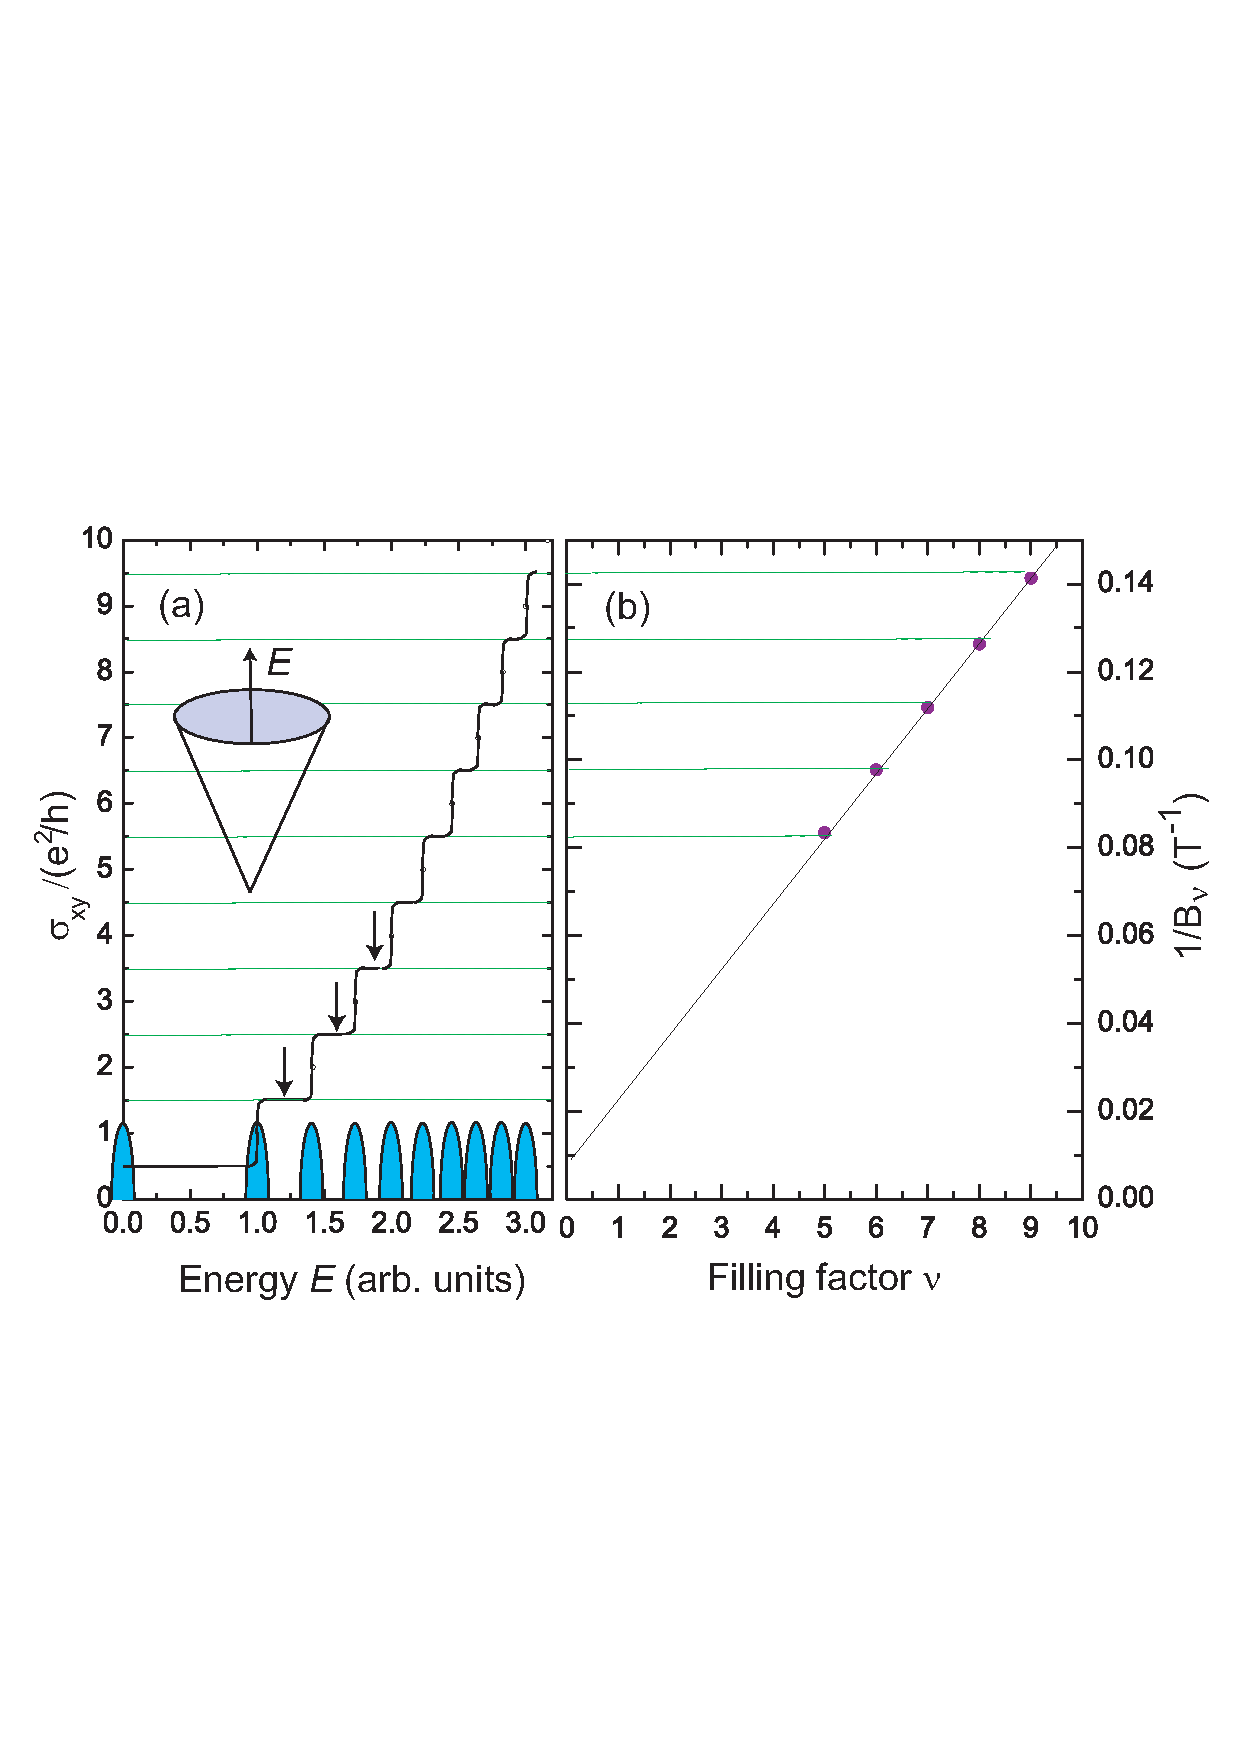
\includegraphics[width=0.9\linewidth]{ch-bts/figures/FigDiracIndex2.pdf} 
\caption{\label{figindex} 
Construction used to fix the filling factors for a Dirac spectrum.  Panel (a) depicts how the Landau indices are decided for a 2D Dirac gas in the quantum Hall regime. It sketches
schematically the step-like increase of $\sigma_{xy} = (e^2/h)[\nu+\frac12]$ versus energy $E$,
where $\frac12$ arises from the $\nu$ = 0 LL at the Dirac point.
The half-ovals are broadened Landau Levels centered at $E_{\nu}=\hbar\ell_B^{-1} v_F\sqrt{2\nu}$.
$B_{\nu}$ are the fields at which $E_F$ falls between LLs (arrows).  The inset
shows the 2D Dirac energy surface in zero $B$.  In Panel (b), we compare this definition of filling factors $\nu$ with
the measured values of $1/B_{\nu}$.
The 5 values of $1/B_{\nu}$ fall on a straight line 
that intercepts the $\nu$ axis at -0.55. The intercept that is close to $\frac{1}{2}$ (mod 1) is consistent with a Dirac spectrum.  
} 
  \end{center}
\end{figure}

Compared to those in Bi$_2$Te$_3$, the SdH oscillations in Bi$_2$Te$_2$Se are much more outstanding. Such prominent oscillations also provide us an opportunity to address whether the surface states' dispersion is Dirac like or not. The previous results on Bi$_2$Te$_3$ have some ambiguity on this issue due to the small amplitudes of the oscillations. In principle, one may plot the
"index" field $1/B_{\nu}$ versus the filling factors $\nu = 1,2 \cdots$, and track the intercept in the limit $B\to\infty$.  Nevertheless, one needs to be careful about whether to take the maxima or minima of $\rho_{xx}$ or $\rho_{yx}$ for the index fields when the sample is not in the quantum Hall regime. Also, as we will discuss in the next subsection, the mixing with a large bulk conductivity will also make this problem even more subtle.  Here we define the index field $B_{\nu}$ as the field at which the chemical potential $E_F$ falls between 2 LLs. The definition could be changed but it should be consistent in $\sigma_{ij}$ and $\rho_{ij}$, and it should agree with the quantum Hall limit as well. With our definition, when the applied field is $B=B_{\nu}$ in the quantum Hall limit, the Hall conductivity has plateau values $\sigma_{xy} = (e^2/h)(\nu+\frac12)$ for the Dirac electrons (compared with $\sigma_{xy} = \nu e^2/h$ for the Schr\"{o}dinger ones). As a result, the index plot n \emph{v.s.} $1/B_{\nu}$ of the Dirac electrons has an intercept of $\frac{1}{2}$ (mod 1) on the $n$-axis, while that of Schr\"{o}dinger electrons intercept 0. In Bi$_2$Te$_2$Se, the large amplitudes could help us determine the "index" field more accurately and thus reduce the uncertainties in the extrapolated intercept.




%%%%%%%%%%%%%%%%%%%%%%%%%%%%%%%%%%%%%%%%
%%%%%%%%%%%%%%%%%%%%%%%%%%%%%%%%%%%%%%%%
%%%%%%%%%%%%%%%%%%%%%%%%%%%%%%%%%%%%%%%%
%%%%%%%%%%%%%%%%%%%%%%%%%%%%%%%%%%%%%%%% FIGURE

\begin{figure}[!htbp]
  \begin{center}            
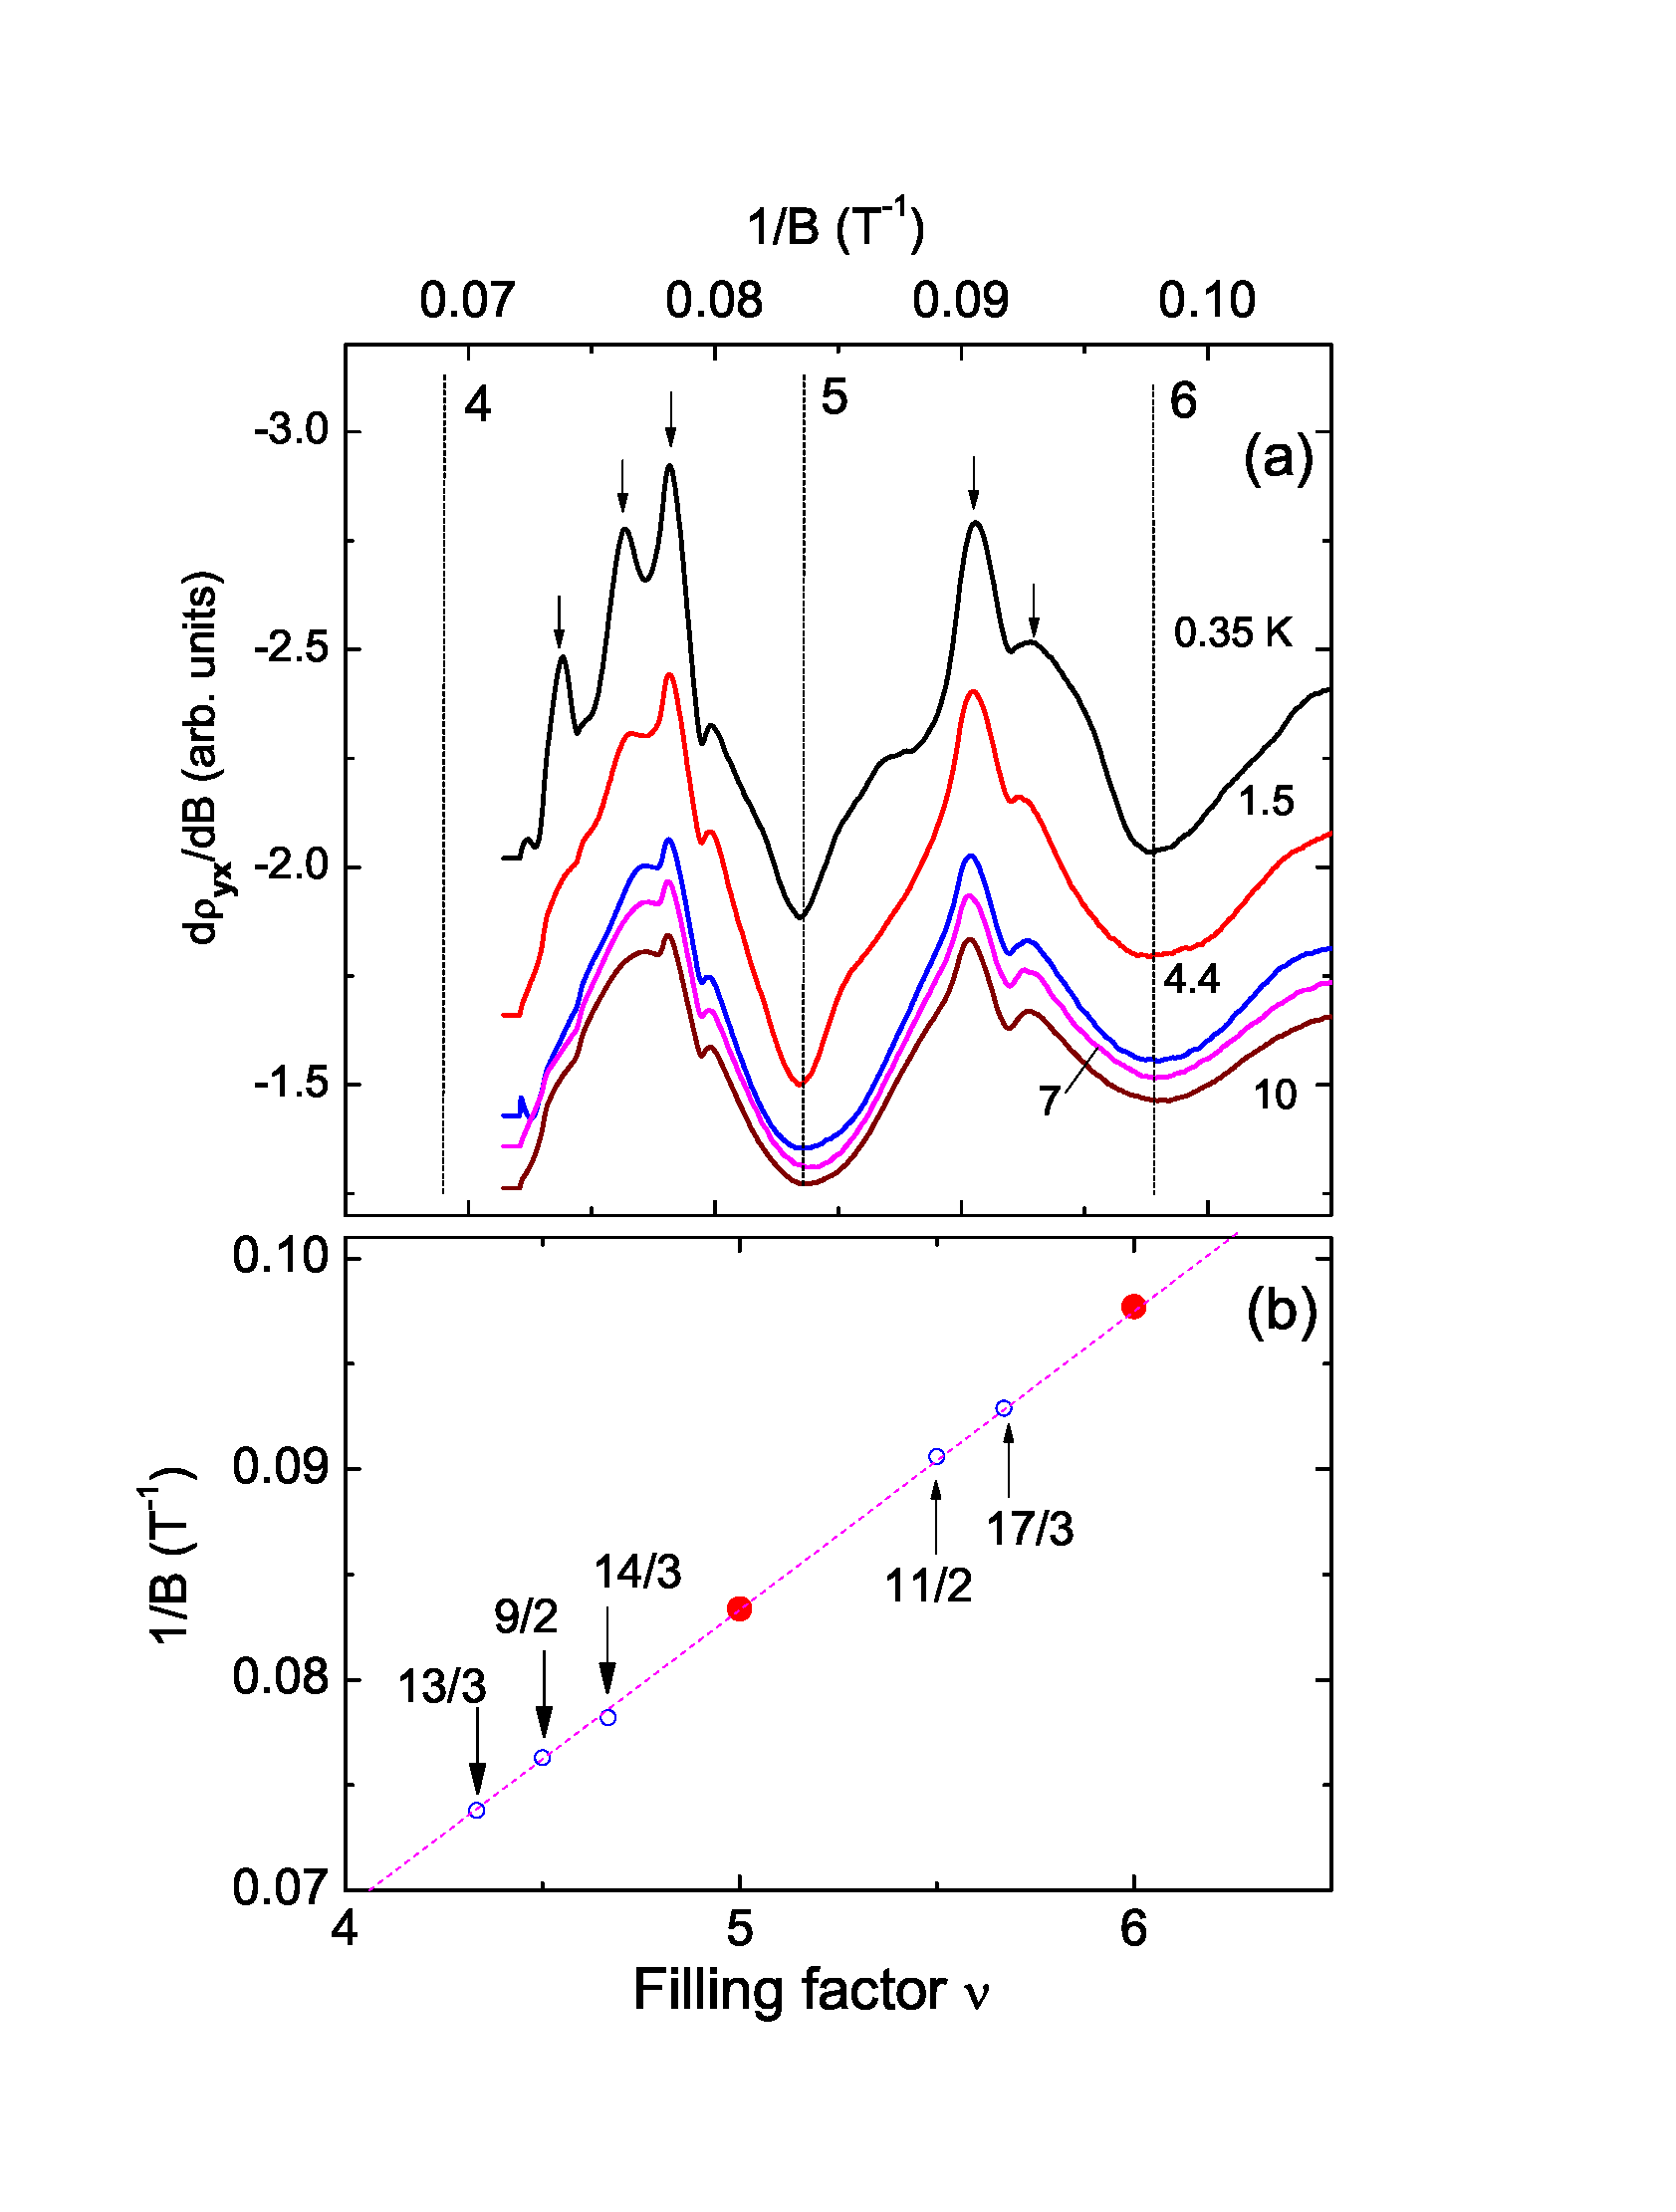
\includegraphics[width=0.9\linewidth]{ch-bts/figures/FigrhoxyExpand.eps} 
\caption{\label{figexpand} 
The possible fractional filling states in the SdH oscillations.
Panel (a): Expanded view of $d\rho_{yx}/dB$ of Bi$_2$Te$_2$Se for 4$<\nu<$6 shows sharp
maxima at non-integer values of $\nu$, at $T$ from 0.35--10 K. The feature decreases rapidly with an increasing temperature. The arrows
locate the more prominent peaks.  In Panel (b), the peak positions plotted
against $\nu$ align well with fractional values of $\nu$ (arrows mark the values
$\nu$ = 13/3, 9/2, $\cdots$, 17/3). 
}
  \end{center}
\end{figure}


Fig. \ref{figindex} is a sketch that relates the index plot ($1/B_{\nu}$ vs. $\nu$) and the Hall plateaus to the Dirac energy spectrum.  
Fig. \ref{figindex}a shows the steps of the quantized Hall conductivity $\sigma_{xy}/(e^2/h)$ versus the Fermi energy $E_F$,  where the shift of $\frac12$ arises from the $\nu = 0$ LL at the Dirac point, as in graphene. The half-ovals drawn on the $E$-axis represent the broadened LLs.  As the density of states (DOS) reaches the peaks at the step-edges of $\sigma_{xy}$, $d\rho_{yx}/dB$ also reaches the maxima. Consequently, the minima in $|d\rho_{yx}/dB|$ locate $B_{\nu}$, the field at which $E_F$ lies between LLs (arrows) as we defined. The $\frac12$-shift of the intercept implies that the line of $1/B_{\nu}$ vs. $\nu$ in Panel (b) does not pass through the origin (whereas it does for a quadratic dispersion).


To find the intercept for our Bi$_2$Te$_2$Se sample, we plot the measured $1/B_{\nu}$ versus $\nu$ in Fig. \ref{figindex}b.
With just one vertical scale adjustment, we can align the 5 data points to the steps in Panel (a).  At our highest $B$, the filling factor is $\nu$ = 5.
The straight line fitted to the data in (b) noticeably intercepts the $\nu$ axis at $\nu$ = -0.55 instead of 0, consistent with the $\frac12$ shift expected from a Dirac spectrum.  

Another possibly interesting point in our data is the additional peaks in the oscillations. Recently, Analytis \etal~\cite{Analytis} reported possibly fractional-filling states in (Bi,Sb)Se$_3$ in very intense fields ($B>$50 T). We also find some similar evidence for fractional-filling states that
emerge at much lower fields (11 T).  Fig. \ref{figexpand}a shows an intriguing array of sharp \emph{maxima} in $d\rho_{yx}/dB$ (arrows) that is apparent for 4$<\nu <$6. The peaks become weaker as $T$ increases from 0.35 K, but some 
are still resolved even at 10 K.  Interestingly, we notice that the peak positions align well with fractional values of $\nu$, as shown in Fig. \ref{figexpand}b. But these fractional features may need more detailed study in samples with higher mobilities. Unfortunately, as we will see in the next subsection, these features do not appear in our samples in a higher magnetic field. Further investigation may needed with samples of higher quality.
